\chapter{Herramientas y dispositivos utilizados}

En este capítulo se cubre todas las herramientas, tanto software como lenguajes de programación o tipos de bases de datos utilizadas, y dispositivos utilizados, que se organizan según su función en la \textit{Smarthome}.

\section{Software utilizado}

El software se divide según su funcionalidad o la parte del trabajo en la que se ha utilizado: durante el desarrollo del proyecto, la escritura de la memoria o la comunicación con los tutores.

\subsection{Desarrollo}

Durante el desarrollo del proyecto se han utilizado multitud de programas, lenguajes y entornos, cada uno llevando a cabo una o varias funcionalidades.

\begin{itemize}
    \item \textbf{Python:} es uno de los lenguajes de programación más populares y potentes de los últimos años. Entre sus características, destacan el tipado dinámico, su flexibilidad para usarse en cualquier ámbito y su amplia librería\cite{cap3_4}, junto a los módulos desarrollados por la comunidad, lo convierten en un lenguaje muy potente e ideal para este trabajo. Permitirá poder gestionar y controlar el resto de entornos y herramientas de manera sencilla a través de distintos scripts.
    \begin{figure}[h]
        \centering
        
\includegraphics[width=3cm]{imagenes/capitulo3/pythonLogo.png}
        \caption{Logotipo de Python.}
        \label{fig:python_logo}
    \end{figure}

    \item \textbf{Visual Studio Code: } es un editor de código muy escalable y personalizable, ya que aunque no está inicialmente orientado para trabajar con Python, en su amplio catálogo de extensiones se encuentra una que compatibiliza el editor con el lenguaje, pudiendo incluso ejecutarlo directamente desde el mismo\cite{cap3_5}. También ofrece otras ventajas como integridad completa con el repositorio de git, del que se hablará a continuación.
    \begin{figure}[h]
        \centering
        
\includegraphics[width=3cm]{imagenes/capitulo3/VisualStudioLogo.png}
        \caption{Logotipo de Visual Studio Code.}
        \label{fig:visualStudioCode_interfaces}
    \end{figure}

    \item \textbf{Git: }es un sistema de control de versiones que ayuda a gestionar el proyecto, restaurar código si fuera necesario o probar distintas modificaciones en paralelo que no afecten a la versión principal \cite{cap3_6}. Es una de las herramientas más potentes para desarrollos tanto por equipos como en solitario. Gracias a GitHub, una extensión de Git donde almacenar el proyecto \textit{online}, el repositorio es más accesible y compartible desde cualquier lugar al permitir el acceso por interfaz web.
    \begin{figure}[h]
        \centering
        
\includegraphics[width=4cm]{imagenes/capitulo3/gitLogo.png}
        \caption{Logo de git.}
        \label{fig:git_logo}
    \end{figure}

    \item \textbf{Docker: }es un software de creación y gestión de contenedores, que se pueden definir como instancias independientes del equipo \textit{host}. Estas instancian se crean a partir de una imagen que puede ser de cualquier sistema operativo y sus correspondientes versiones o sistemas ya preparados para ejecutar software y programas específicos, como los utilizados en este trabajo.
    \begin{figure}[h]
        \centering
        
\includegraphics[width=4cm]{imagenes/capitulo3/dockerLogo.png}
        \caption{Logo de Docker.}
        \label{fig:docker_logo}
    \end{figure}

    \item \textbf{MongoDB: }es una base de datos basada en documentos, unas estructuras de datos compuesto por pares de campo y valor, que a su vez se almacenan en colecciones, similar a lo que en bases de datos relacionales son las tablas. La elección de mongoDB se debe a la sencilla integración con Python y a la velocidad y eficienza de almacenamiento y recuperación de datos, gracias a su sistema de colecciones.
    \begin{figure}[h]
        \centering
        
\includegraphics[width=6cm]{imagenes/capitulo3/mongoDBLogo.png}
        \caption{Logo de MongoDB.}
        \label{fig:mongodb_logo}
    \end{figure}

    \item \textbf{InfluxDB: }es una base de datos de series temporales, es decir, los datos se organizan por horas. Al igual de MongoDB, InfluxDB tiene una integración sencilla con Python, también es una de las bases de datos más usadas en el campo del Internet de las cosas gracias a la facilidad que supone monitorear y visualizar los datos guardados en ella.
    \begin{figure}[h]
        \centering
        
\includegraphics[width=6cm]{imagenes/capitulo3/influxDBLogo.png}
        \caption{Logo de InfluxDB.}
        \label{fig:influxdb_logo}
    \end{figure}

    \item \textbf{Grafana: }es un potente software al que se accede por interfaz web que permite monitorizar a través de paneles personalizables los datos registrado en InfluxDB. Su elección viene a partir de que el contenedor para Docker utilizado ya tiene InfluxDB integrado con Grafana, lo que facilita la comunicación de ambos software. Además de que permite trabajar de forma dinámica con diferentes rangos de tiempo, permite mostrar gráficos a tiempo real y tiene una avanzada personalización del panel donde se muestra toda la información.
    \begin{figure}[h]
        \centering
        
\includegraphics[width=3cm]{imagenes/capitulo3/GrafanaLogo.png}
        \caption{Logo de Grafana.}
        \label{fig:grafana_logo}
    \end{figure}
    
\end{itemize}

\subsection{Comunicación}
Para la comunicación con los tutores, se han usado principalmente el intercambio de correos electrónicos a través de Gmail y, también otro servicio de Google, Meet para las reuniones en videollamada.
\begin{figure} [h]
     \centering
     \begin{subfigure}[b]{.35\textwidth}
         \centering
         
\includegraphics[width=\textwidth]{imagenes/capitulo3/GmailLogo.png}
         \caption{Logo de Gmail.}
         \label{fig:gmail_logo}
     \end{subfigure}
     \hfill
     \begin{subfigure}[b]{.55\textwidth}
         \centering
         
\includegraphics[width=\textwidth]{imagenes/capitulo3/MeetLogo.png}
         \caption{Logo de Meet.}
         \label{fig:meet_logo}
     \end{subfigure}
\end{figure}

\subsection{Memoria}
La memoria ha sido escrita utilizando Overleaf, un editor de textos online y colaborativo. Este editor se enfoca en escribir un Latex que es una herramienta de redacción de documentos científicos y profesionales.
\begin{figure}[h]
        \centering
        
\includegraphics[width=5.5cm]{imagenes/capitulo3/Overleaf_logo.png}
        \caption{Logo de Overleaf.}
        \label{fig:overleaf_logo}
    \end{figure}
Su funcionamiento es algo diferente respecto al resto de editores de texto. En lugar de escribir un texto y luego formatear con los distintas herramientas del editor, en Latex se utilizando comando para formatear automáticamente el apartado que se vaya a escribir. De esta manera se mantiene un orden y formato a lo largo de todo el documento, siguiendo cada apartado unos reglas especificadas para cada comando.

\section{Dispositivos de la \textit{Smarthome}}

Como se ha explicado en el capítulo 2, los dispositivos de la \textit{Smarthome} podemos dividirlos entre sensores, actuadores y dispositivos con funcionalidades más concretas. Para el desarrollo del TFG se han utilizado distintos dispositivos, principalmente sensores, actuadores y la unidad central de la \textit{Smarthome}.

\subsection{Unidad central}

Como se comentó anteriormente, la Smarthome cuenta con un servidor web que actúa como unidad central del sistema. Este dispositivo es el SpaceLynk LSS100200, desde el que se puede controlar a través de su interfaz web o de su API los valores de todos los dispositivos del sistema, añadir aplicaciones compatibles o incluso programar procedimientos simples\cite{cap3_1}.

\begin{figure}[h]
    \centering
    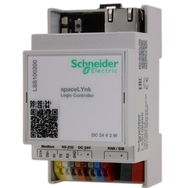
\includegraphics{imagenes/capitulo3/SpaceLynk_dispositivo.jpg}
    \caption{Dispositivo SpaceLynk LSS100200.}
    \label{fig:spacelynk_dispositivo}
\end{figure}

Se pueden acceder a sus distintas funcionalidades a través del navegador, utilizando la IP del servidor. Tras iniciar sesión, se mostrarán todas las opciones disponibles:

\begin{figure}[h]
    \centering
    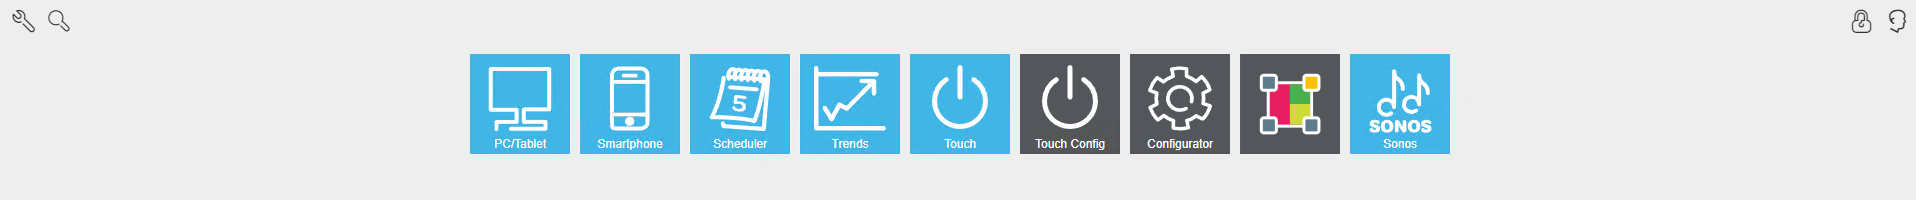
\includegraphics[width=1\textwidth, keepaspectratio]{imagenes/capitulo3/menuSpaceLynk.png}
    \caption{Menú principal del SpaceLynk.}
    \label{fig:spacelynk_menu}
\end{figure}

\begin{itemize}
    \item \textbf{Interfaz de PC/Tablet:} consiste en una interfaz que representa las habitaciones de la Smarthome junto a su mayoría de sensores y actuadores, sobre los que se pueden modificar su estado o valor para encender luces, levantar persianas y otras funcionalidades.
    \begin{figure}[h]
        \centering
        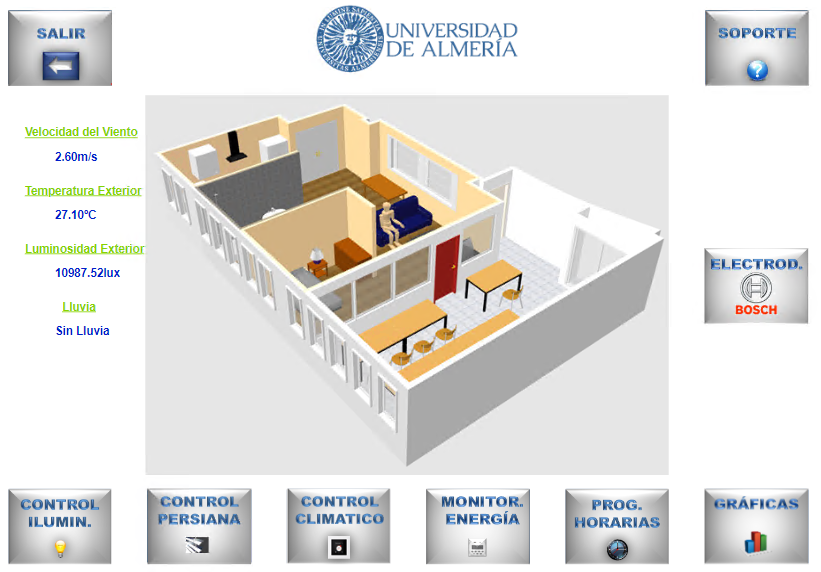
\includegraphics[width=0.8\textwidth, keepaspectratio]{imagenes/capitulo3/interfazPC.png}
        \caption{Interfaz de control para PC y tablets.}
        \label{fig:interfazPC}
    \end{figure}
    \item \textbf{Interfaz de Smartphone:} tiene la misma funcionalidad que la interfaz para PC/Tablet, salvo que tiene un diseño basado en menús y desplegables.
    \begin{figure}[h]
        \centering
        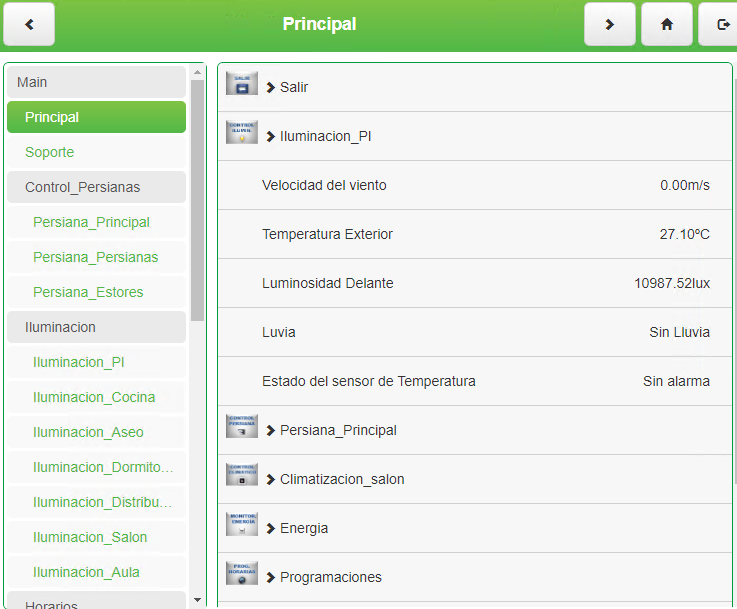
\includegraphics[width=0.8\textwidth, keepaspectratio]{imagenes/capitulo3/interfazMovil.png}
        \caption{Interfaz de control para Smartphones.}
        \label{fig:interfaz_smartphones}
    \end{figure}
    \item \textbf{\textit{Scheduler}:} más que una funcionalidad, es un acceso directo a la sección homónima del apartado de configuración. Permite gestionar periodos de tiempo específicos en el calendario. Así, se podrán asignar acciones diferentes a la Smarthome en función de la época del año.
    \item \textbf{\textit{Trends}:} al igual que la anterior, es un acceso directo que apunta a su respectiva sección del apartado de configuración. Permite visualizar las gráficas de los valores de sensores, u otros dispositivos con valores representables, en un intervalo de tiempo específico.
    \begin{figure}[h]
        \centering
        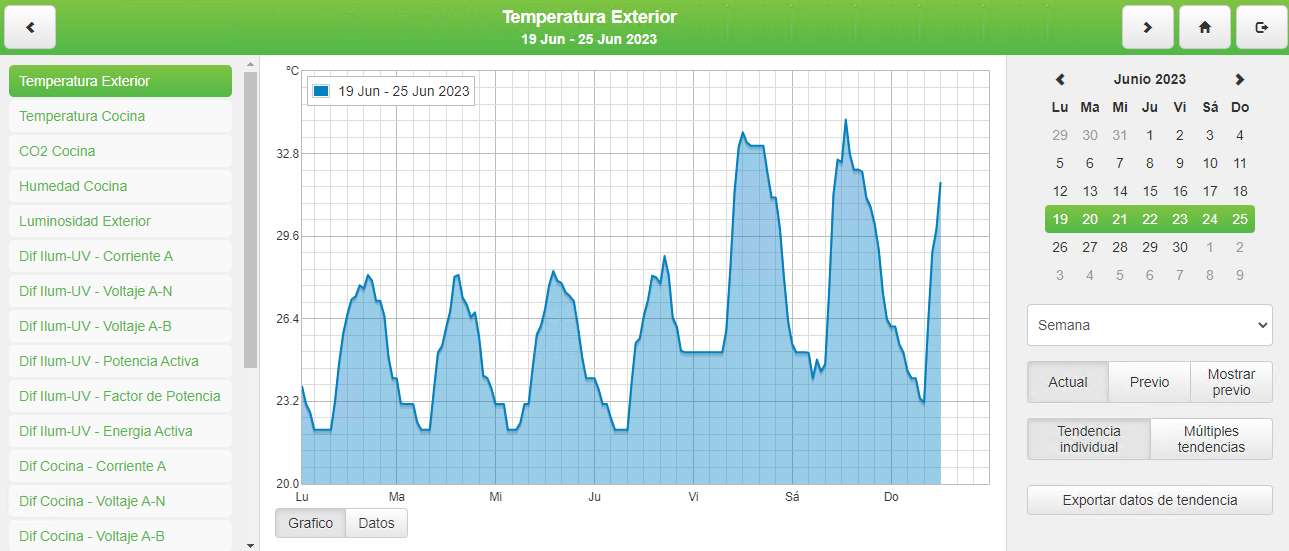
\includegraphics[width=0.8\textwidth, keepaspectratio]{imagenes/capitulo3/interfazTrends.png}
        \caption{Interfaz de los registros de tendencias.}
        \label{fig:interfaz_trends}
    \end{figure}
    \item \textbf{\textit{Touch}/\textit{Touch Config}:} esta función permite diseñar de forma sencilla interfaces para poder realizar acciones sobre los dispositivos de la Smarthome o bien para representar sus estados y valores. Estas interfaces están pensadas para ser utilizadas en dispositivos \textit{Touch}, tales como pantallas táctiles que puedan estar adheridas a la pared de una habitación y realizar todo el control de la sala desde la misma. Incluye \textit{widgets}, que son componentes gráficos que suelen cumplir funciones específicas y sencillas, para facilitar aún más el diseño de estas interfaces.
    \begin{figure}[h]
        \centering
        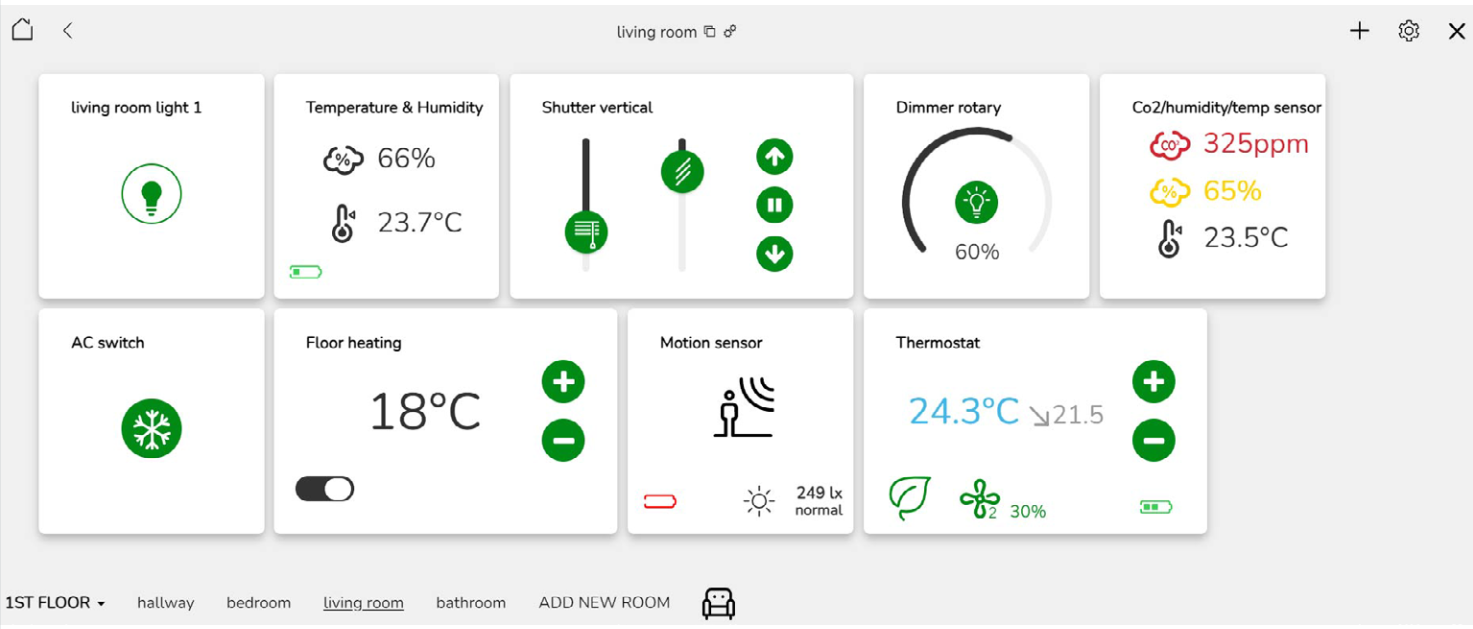
\includegraphics[width=0.8\textwidth, keepaspectratio]{imagenes/capitulo3/interfazTouch.png}
        \caption{Interfaz Touch de ejemplo.}
        \label{fig:interfaz_touch}
    \end{figure}
    \item \textbf{Configurador:} esta es la funcionalidad más importante del SpaceLYnk, ya que nos permitirá configurar y gestionar todo el sistema. Además de crear los \textit{Scheduler} o \textit{Trends} que hemos visto antes, podemos gestionar todos los dispositivos conectados al bus, realizar copias de seguridad o resutar el sistema a partir de una, diseñar interfaces como la de PC o Smarthome, programar funciones sencillas en las que actuaremos sobre los dispositivos, etc.
    \begin{figure}[h]
        \centering
        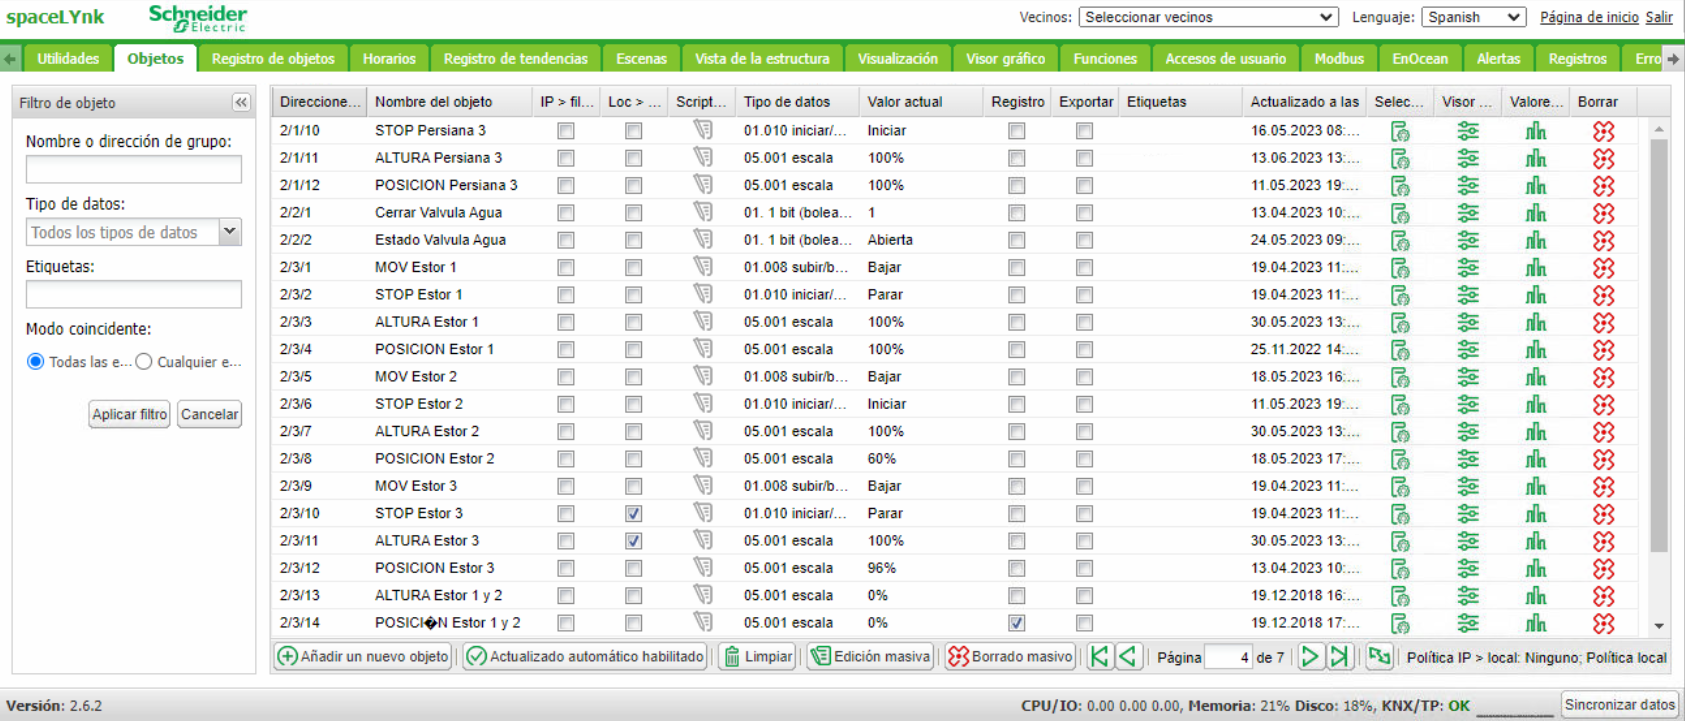
\includegraphics[width=0.8\textwidth, keepaspectratio]{imagenes/capitulo3/InterfazConfigurador.png}
        \caption{Listado de los dispositivos conectados al bus a través de la interfaz del configurador.}
        \label{fig:interfaz_touch}
    \end{figure}
\end{itemize}

\subsection{Sensores}

Los sensores han tomado un papel crucial para el desarrollo de este TFG, ya que han sido los dispositivos que han aportados continuamente todos los datos atmosféricos. Para seleccionar estos sensores, fue necesario estudiar el listado completo en la Smarthome desde el apartado de configurador del SpaceLynk. Cada sensor tiene una dirección de grupo asignada, que actúa como una dirección IP en una LAN, pero dentro del bus KNX. Sin embargo, esto no significa que haya un dispositivo físico para cada sensor, sino que es común que un mismo dispositivo físico se encarga de medir varios de estos valores. Este es el listado de los sensores utilizados:

\begin{itemize}
    \item \textbf{KNX - Estación meteorológica básica V2 (MTN6904-0001): }esta estación meteorológica no actúa como un único sensor, sino que dispone de sensor de temperatura (exterior), luminosidad, velocidad del viento y de lluvia \cite{cap3_2}. Este dispositivo se encarga de tomar las medidas del exterior.
    \item \textbf{KNX - Sonda temperatura, humedad y CO2 (MTN6005-0001): }este dispositivo también dispone de varios sensores, específicamente de temperatura (interior), humedad relativa y CO2 \cite{cap3_3}. Este dispositivo se encarga de tomar las medidas del interior.
\end{itemize}

\begin{figure}[h]
    \begin{subfigure}{0.5\textwidth}
        \centering
        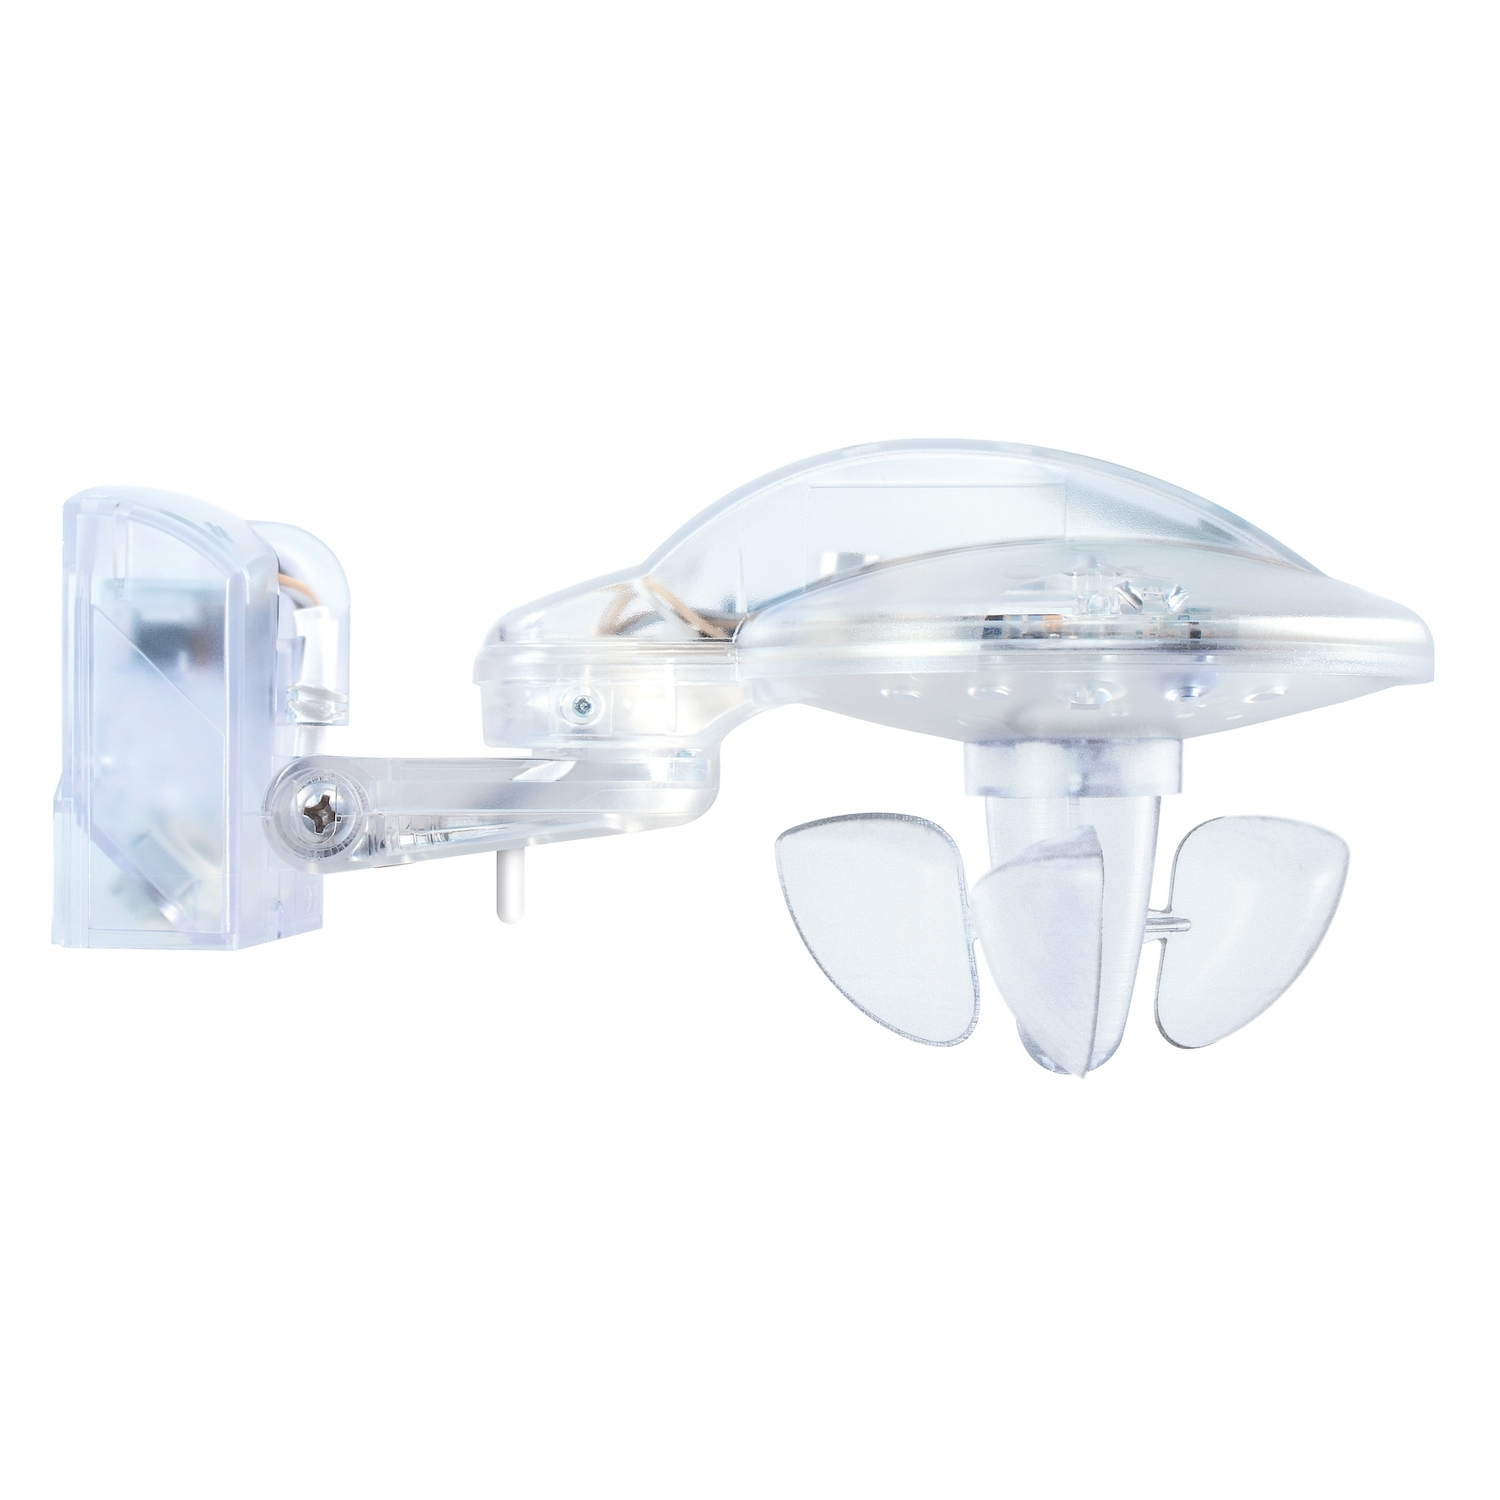
\includegraphics[width=0.9\textwidth, keepaspectratio]{imagenes/capitulo3/estacionMeteorologica.jpg}
        \caption{Dispositivo MTN6904-0001}
        \label{fig:estacionMeteorologica}
    \end{subfigure}
    \begin{subfigure}{0.5\textwidth}
        \centering
        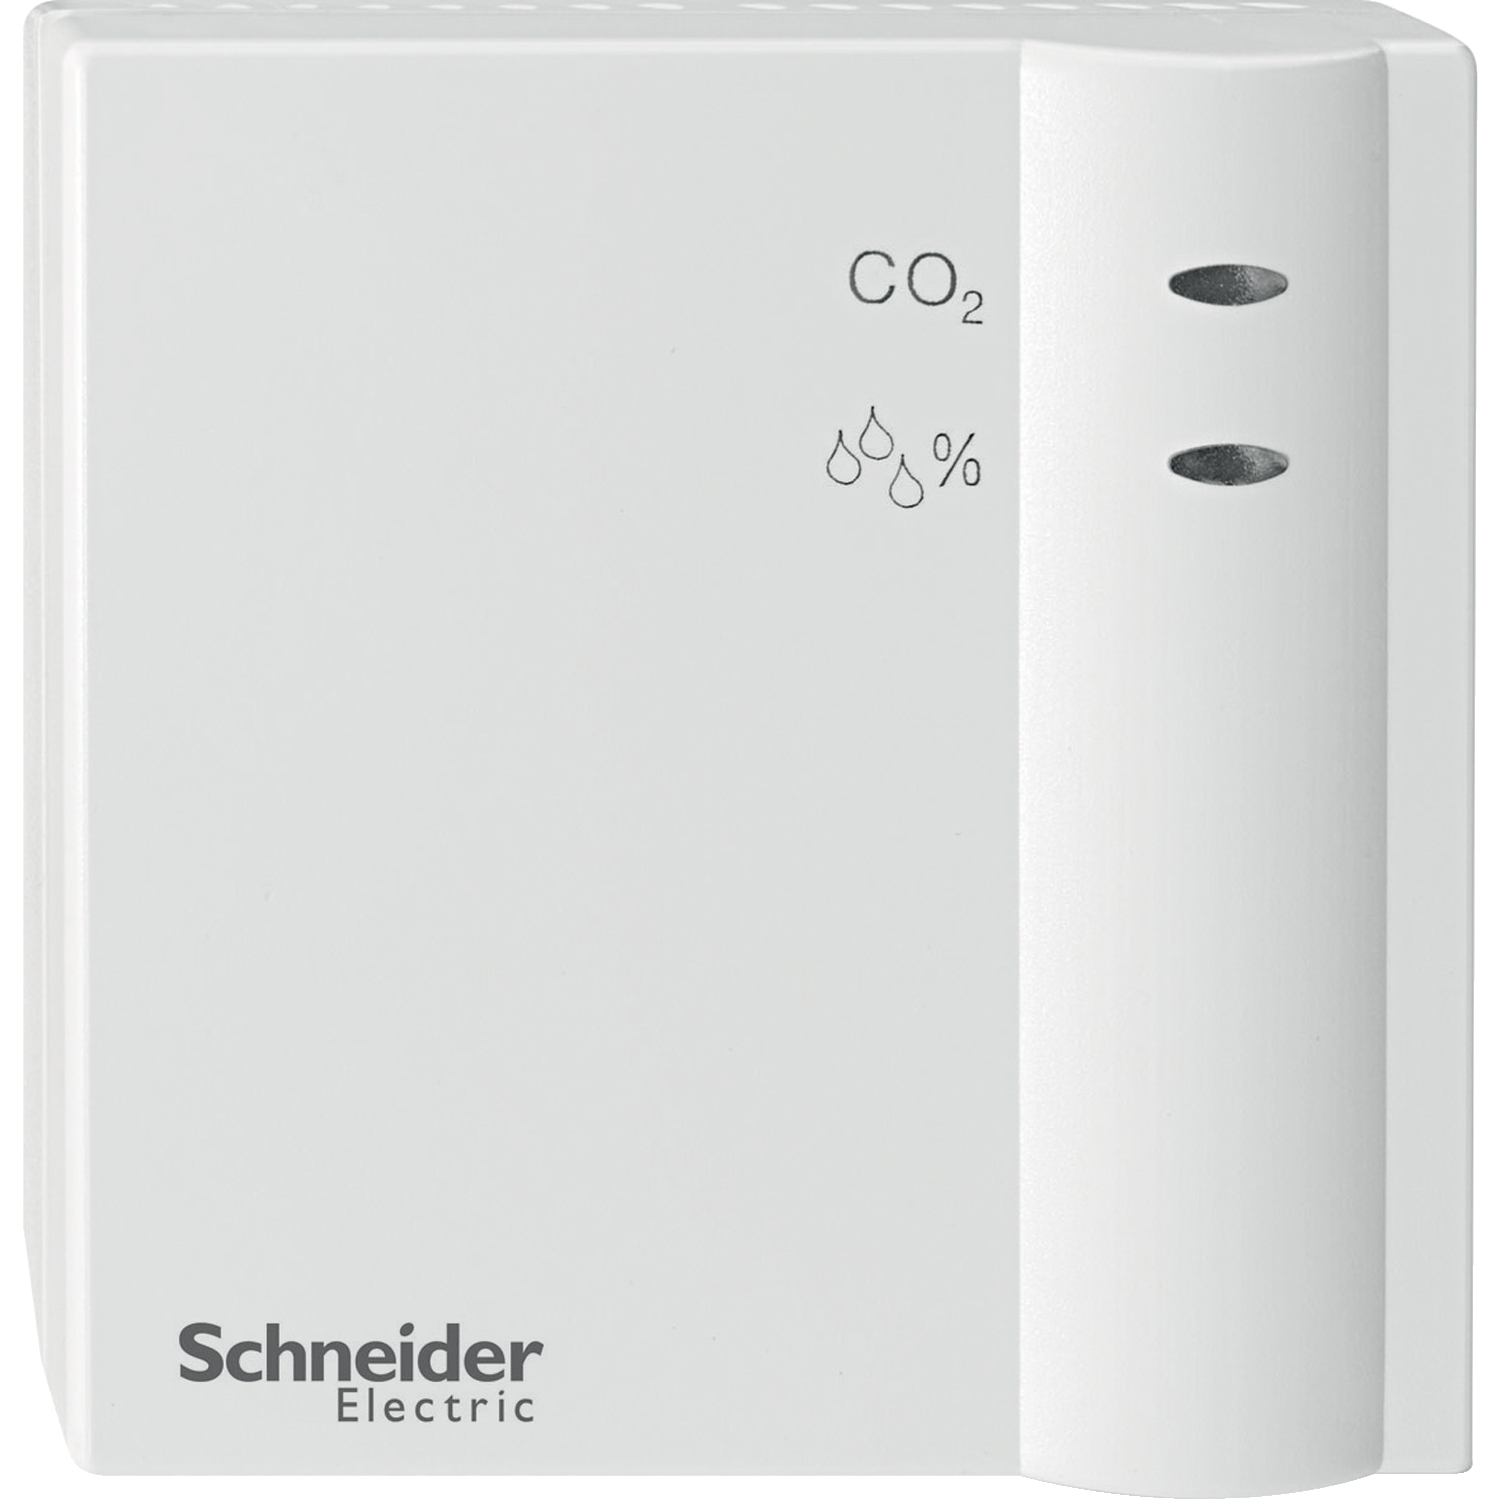
\includegraphics[width=0.9\textwidth, keepaspectratio]{imagenes/capitulo3/sondaTempHumeCO2.jpg}
        \caption{Dispositivo MTN6005-0001}
        \label{fig:sondaParametrosInterior}
    \end{subfigure}
\end{figure}

En total, son siete parámetros atmosféricos los que se van a medir constantemente en este trabajo y sobre los que se va a basar el sistema de control de confort térmico.



\subsection{Actuadores}